%%%
%
% $Autor: Gargi Barve $
% $Date: 2024-10-31 11:15:45Z $
% $File: file.tex $
% $Version: 1 $
%
% Project: 
%
%%%

\chapter{Scikit-learn}
\label{ch:scikit}

\section{Introduction}

\textbf{Scikit-learn} is an open-source Python library for machine learning and model evaluation. In this CPI forecasting project, it is not used for model training itself, because the forecasting models are estimated with \textbf{statsmodels}. Its importance instead lies in the \textbf{evaluation layer} of the workflow. The library provides the metric functions that make the comparison between ARIMA, ETS, and SARIMA consistent, transparent, and reproducible \cite{scikit-learn-doc}.

This illustrates a selective but academically relevant use of a software package. Although \textbf{scikit-learn} is not the forecasting engine of the system, it provides the numerical basis for judging forecast quality on the chronological holdout period.

\section{Description}

The project uses \textbf{scikit-learn} in a focused way through the module \textbf{sklearn.metrics}. In \FILELOC{Code/src/modeling\_pipeline.py}, the functions \textbf{mean\_squared\_error}, \textbf{mean\_absolute\_error}, and \textbf{mean\_absolute\_percentage\_error} are applied to compare predicted CPI values against the actual CPI values in the 24-month test set. The same metric logic is also used again in \FILELOC{Code/app.py} so that the dashboard displays evaluation values consistent with the offline modeling pipeline.

This role is directly aligned with the project objective. Since the task is to compare three forecasting models under one common setup, the evaluation package must deliver standardized and interpretable metrics. \textbf{Scikit-learn} fulfills this requirement well because its metric functions are widely used, stable, and easy to integrate with \textbf{pandas}- and \textbf{numpy}-based workflows.

Table~\ref{tab:sklearn-metrics-role} summarizes the role of the three evaluation metrics used in this project.

\begin{table}[htbp]
	\centering
	\caption{Interpretation of scikit-learn metrics in the CPI forecasting project.}
	\label{tab:sklearn-metrics-role}
	{\small
	\renewcommand{\arraystretch}{1.22}
	\setlength{\tabcolsep}{7pt}
	\begin{tabular}{L{2.4cm}L{5.4cm}L{5.5cm}}
		\hline
		Metric & What it measures & Why it matters in this project \\
		\hline
		RMSE & Square-rooted average of squared forecast errors & Penalizes larger CPI forecast misses more strongly and is therefore useful when substantial deviations are especially undesirable \\
		MAE & Average absolute forecast deviation & Provides a direct interpretation in CPI index points and is easy to compare across models \\
		MAPE & Average percentage forecast deviation & Supports scale-relative comparison and improves interpretability for non-technical readers \\
		\hline
	\end{tabular}
	}
\end{table}

\section{Installation}

The project records \textbf{scikit-learn} as a dependency in \FILELOC{Code/requirements.txt}. Installation is therefore handled together with the other Python packages used in the repository:

\begin{Python}[caption={Installing project dependencies including scikit-learn}, label={lst:install_sklearn_project}]
	pip install -r Code/requirements.txt
\end{Python}

If scikit-learn must be installed separately, the package manager command is:

\begin{Python}[caption={Installing scikit-learn directly}, label={lst:install_sklearn_direct}]
	pip install scikit-learn
\end{Python}

The installation can be verified with a short version check:

\begin{Python}[caption={Verifying the scikit-learn installation}, label={lst:verify_sklearn}]
	import sklearn
	print(sklearn.__version__)
\end{Python}

\section{Example -- Description}

A concrete repository example is the evaluation of the three forecasting models on the holdout period. After ARIMA, ETS, and SARIMA generate their 24-step forecasts, scikit-learn metrics are used to measure how far these predictions deviate from the actual CPI values. The resulting metrics answer complementary questions:

\begin{itemize}
	\item \textbf{RMSE} emphasizes larger forecast errors more strongly.
	\item \textbf{MAE} gives the average absolute forecast error in CPI index points.
	\item \textbf{MAPE} expresses the error in percentage terms and supports intuitive comparison.
\end{itemize}

For the current repository version, this evaluation shows that the ETS model performs best, with RMSE $= 0.7697$, MAE $= 0.6453$, and MAPE $= 0.5298\%$. These values are taken from the exported evaluation results in \FILELOC{Code/plots/evaluation\_metrics.csv}.

\section{Example -- Manual}

The scikit-learn-based evaluation can be reproduced with the following project-specific steps:

\begin{enumerate}
	\item Install the dependencies from \FILELOC{Code/requirements.txt}.
	\item Ensure that the dataset \FILELOC{Code/data/61111-0002\_en.csv} is present.
	\item Run \FILELOC{Code/src/modeling\_pipeline.py} from the \FILELOC{Code} directory.
	\item Let the pipeline train ARIMA, ETS, and SARIMA on the training data.
	\item Inspect the printed metric output and the exported file \FILELOC{Code/plots/evaluation\_metrics.csv}.
	\item Optionally start \FILELOC{Code/app.py} with \textbf{Streamlit} and compare the same metrics in the dashboard.
\end{enumerate}

\section{Example -- Code}

Listing~\ref{lst:sklearn_project_metrics} shows the actual type of scikit-learn usage employed in the project.

\begin{Python}[caption={Forecast evaluation with scikit-learn metrics}, label={lst:sklearn_project_metrics}]
	from sklearn.metrics import (
	mean_squared_error,
	mean_absolute_error,
	mean_absolute_percentage_error
	)
	import numpy as np
	
	rmse = np.sqrt(mean_squared_error(test['CPI'], preds))
	mae = mean_absolute_error(test['CPI'], preds)
	mape = mean_absolute_percentage_error(test['CPI'], preds) * 100
\end{Python}

This code is repository-relevant because it matches the implementation in \FILELOC{Code/src/modeling\_pipeline.py} and is reused conceptually in \FILELOC{Code/app.py} to ensure consistency between offline evaluation and dashboard display.

\section{Example -- Files}

The main files in which scikit-learn is used are:

\begin{itemize}
	\item \FILELOC{Code/src/modeling\_pipeline.py} -- computes RMSE, MAE, and MAPE during offline evaluation.
	\item \FILELOC{Code/app.py} -- recomputes the same metrics for display in the Streamlit dashboard.
	\item \FILELOC{Code/plots/evaluation\_metrics.csv} -- stores the metric results generated from these computations.
\end{itemize}

\section{Package Role in the CPI Pipeline}

The following figure is not a second full methodology diagram, but a focused view of where \textbf{scikit-learn} enters the repository workflow. Relative to Chapter~\ref{ch:kdd-methodology}, it belongs mainly to the \textbf{interpretation and evaluation stage}. After the forecasting models have produced predictions for the test horizon, these predicted values are compared with the corresponding \textbf{actual CPI holdout values}. \textbf{Scikit-learn} then converts this comparison into RMSE, MAE, and MAPE values that can be evaluated consistently across ARIMA, ETS, and SARIMA. The figure is therefore meant to clarify the package's analytical role rather than to compete with the broader KDD structure.

\begin{figure}[htbp]
	\centering
	\resizebox{0.95\linewidth}{!}{
		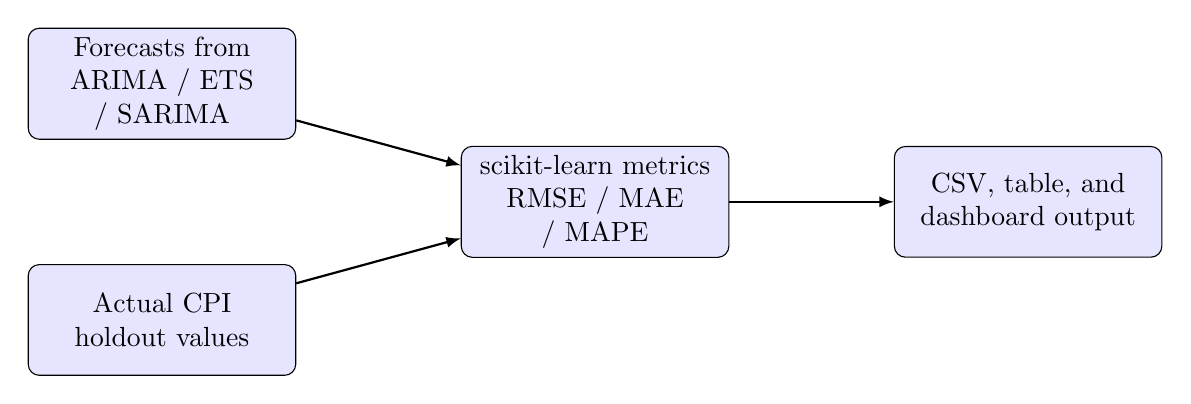
\begin{tikzpicture}[
    block/.style={rectangle, draw, fill=blue!10, text width=9em, text centered, rounded corners, minimum height=4em},
    line/.style={draw, -latex, thick}
    ]
    \node [block] (forecast) at (0,1.5) {Forecasts from\\ARIMA / ETS / SARIMA};
    \node [block] (actual) at (0,-1.5) {Actual CPI\\holdout values};
    \node [block] (metric) at (5.5,0) {scikit-learn metrics\\RMSE / MAE / MAPE};
    \node [block] (output) at (11,0) {CSV, table, and\\dashboard output};
    
    \draw [line] (forecast) -- (metric);
    \draw [line] (actual) -- (metric);
    \draw [line] (metric) -- (output);
\end{tikzpicture}
}
	\caption{Package-level view of \textbf{scikit-learn} within the CPI pipeline. In KDD terms, the figure corresponds mainly to the interpretation and evaluation stage, where model forecasts and actual holdout values are converted into comparable performance metrics.}
	\label{fig:sklearn_workflow}
\end{figure}

\section{Further Reading}

\begin{itemize}
	\item Scikit-learn documentation: \URL{https://scikit-learn.org/stable/index.html}
	\item Metrics and scoring guide: \URL{https://scikit-learn.org/stable/modules/model_evaluation.html}
	\item Pedregosa et al., \textit{Scikit-learn: Machine Learning in Python}
\end{itemize}
